\documentclass[10pt,twocolumn]{article}
\usepackage[margin=0.75in,columnsep=0.25in]{geometry}
\usepackage{times}
\usepackage{graphicx}
\usepackage{booktabs}
\usepackage{amsmath}
\usepackage[numbers,sort&compress]{natbib}
\usepackage[hidelinks]{hyperref}
\usepackage{xcolor}
\newcommand{\todo}[1]{\textcolor{red}{[TODO: #1]}}

\title{When VLM Judges Fail at 3D:\\Validating Layout Judges for Image-Conditioned Scene Generation}
\author{Anonymous submission}
\date{}

\begin{document}
\maketitle

\begin{abstract}
Agentic pipelines that turn reference images into editable 3D scenes increasingly rely on a vision-language model (VLM) to score their
intermediate layouts. They use these scores to accept a layout and to steer its repair. We ask whether such a judge tracks the
quantity it is meant to measure, which is whether objects sit where the reference image puts them in 3D. On a ground-truth benchmark
built from Hypersim interiors and procedurally generated voxel scenes, a production VLM space judge is stable across repeated calls.
It is nonetheless \emph{negatively} correlated with ground truth on real interiors: anchored object recall $\rho=-0.31$, and centre error
$\rho=+0.62$ $[+0.06,+0.90]$ on scenes with enough objects to measure. A 2D landmark-alignment residual fails in the same way.
We trace both failures to \emph{projection-consistent 3D errors}: when the camera field of view or object depth is wrong, objects can
still project into the right image boxes, so any judge that compares reference and render in the image plane rewards the error.
A simple measured judge closes the gap. It compares each landmark's graybox position, seen from the reference camera, with an
off-the-shelf monocular point map of the reference image (object3d). Validated against label-free per-object ground truth from
Hypersim depth and instance masks, it reaches $\rho=0.84$ $[0.74,0.90]$ per landmark and $0.75$ $[0.40,0.91]$ per scene. It ranks
11 of 12 known-worse layouts correctly, and it holds on 13 newly generated rounds ($\rho=0.79$). Deployed as the graybox gate of an
agentic pipeline, it drives repairs that ground truth confirms. On the hardest scene the error falls from 0.77 to 0.23. We also show
that a common evaluation target, label-matched object recall, breaks on scenes with few objects. We therefore argue that layout judges
should be validated against per-object, label-free truth before they are trusted to guide generation.
\end{abstract}

\section{Introduction}
Recent systems build 3D scenes from one or two reference images by planning a layout, building a coarse \emph{graybox}, and refining it
with multimodal models in a loop~\cite{scenelm,sceneconductor,scenepilot}. Because the loop needs a signal before ground truth exists,
many systems ask a VLM to compare rendered views with the references and score the result. The same score usually decides whether a
layout is accepted and which way a repair should go. If the judge is wrong, every repair it steers is a guess.

Prior work has shown that VLM judges of 3D content are sensitive to the rendered viewpoint~\cite{scenecritic}, and that they are near
chance on ambiguous geometric contrasts~\cite{crossmodeljudge}. We report a stronger and more specific failure. On image-conditioned
scene generation, a VLM space judge can be \emph{anti-correlated} with 3D correctness, and the reason is structural rather than
noise. This paper makes four contributions:
\begin{itemize}\setlength\itemsep{1pt}
\item A ground-truth benchmark of 39 image-conditioned scenes (Hypersim interiors~\cite{hypersim} and procedurally generated voxel
scenes) with a scorer for layouts, cameras and objects, and a protocol for validating judges against it (\S\ref{sec:bench}).
\item Evidence that a production VLM space judge and a 2D landmark residual both run against ground truth on real interiors. We give
the mechanism, projection-consistent 3D errors, and show that the usual label-matched recall target hides the signal on sparse scenes
(\S\ref{sec:fail}).
\item object3d, a measured layout judge assembled from standard monocular-geometry practice~\cite{moge2,furnset,mirascene}. We validate
it per landmark, per scene, on known-worse perturbations and on new generations (\S\ref{sec:object3d}).
\item A deployment study. As the acceptance gate of an agentic graybox loop, object3d steers repairs toward layouts that ground truth
confirms are better. Deployment also exposed pipeline defects that the old judge had masked (\S\ref{sec:loop}).
\end{itemize}
We do not claim the measurement itself as new. Back-projecting monocular point maps and aligning them per object is how several
reconstruction methods fit layouts~\cite{furnset,mirascene,easy3dfy}. Our claim concerns \emph{evaluation}: which judges can be
trusted, how to tell, and what changes when the trusted one drives generation.

\section{Related work}
\paragraph{LLM/VLM-driven 3D scene generation.} Text-driven systems compose scenes from scene graphs or programs~\cite{scenecraft,holodeck}.
Image-conditioned systems recover metric layouts or orchestrate agents from a single image~\cite{scenelm,sceneconductor}, and some
repair layouts in a grow-and-repair loop~\cite{scenepilot}. Several of them use VLM scores for evaluation or selection.
\paragraph{Judging 3D scenes.} SceneCritic replaces VLM scoring with a symbolic evaluator for text-driven indoor synthesis and shows that
VLM scores change with viewpoint~\cite{scenecritic}. Fine-grained constraint verification exposes identification and attribute errors of
VLM-as-a-judge~\cite{apples}. A cross-model VLM protocol for single-image meshes is above chance only on visible defects~\cite{crossmodeljudge}.
Ground-truth-free consistency metrics built on 3D foundation models, such as MEt3R, inherit the behaviour of their backbone~\cite{oneScene}.
\paragraph{Monocular geometry.} Monocular depth and point-map models~\cite{dav2,moge2} and multi-view reconstructors~\cite{dust3r} now
provide reliable relative geometry and intrinsics. Per-object alignment of such point maps is used to \emph{fit} layouts~\cite{furnset,mirascene,easy3dfy}.
We use it to \emph{judge} them, and we validate that use.

\section{Benchmark and validation protocol}\label{sec:bench}
\paragraph{Scenes.} Set A has 19 Hypersim~\cite{hypersim} interiors with two reference views each, chosen for overlap and object
content. One staircase scene with two scored objects is excluded. Set B has 20 procedurally generated voxel scenes rendered from two
isometric (orthographic) views. Scored objects are those visible in at least 0.5\% of a view's pixels and at least 0.15\,m long.
\paragraph{Scorer.} A planar similarity (scale, yaw, translation) aligns prediction to ground truth. It is initialised from cameras and,
independently, from a label-agnostic RANSAC on object centres. Hungarian matching uses a 1\,m radius and a 0.5\,m penalty for a label
mismatch. We report best-fit recall and \emph{anchored} recall, which keeps the camera-initialised fit and so measures the layout as seen
from the reference cameras. Camera errors relative to the room are reported only when at least three objects match. Alignment-free
pair errors (relative rotation, baseline direction) are always reported. Object metrics enter set statistics only for scenes with at
least 8 scored objects (13 of 18). Below that, recall moves in steps of $1/7$ or more and the room fit is often unreachable.
\paragraph{Label-free per-object truth.} Hypersim provides depth and instance masks for each reference frame. For every landmark whose
observation box matches a scored ground-truth instance (box IoU $\ge 0.5$), we compute the median ground-truth 3D point of that
instance in the camera frame, $p_{gt}$. We compare it with the median graybox ray hit on the landmark's bound instances, $p_g$, after one
scale per view. The truth error is $\|s\,p_g-p_{gt}\|/\|p_{gt}\|$ (capped at 1), and an invisible bound instance scores 1. This target
needs no class labels, and it measures exactly what a layout judge should see.
\paragraph{Judge checks.} (i) Repeatability: three repeated calls on four scenes. (ii) Known-order pairs: recorded grayboxes against
degraded copies, namely objects rotated $20^\circ$, scaled $1.5\times$, 30\% dropped, and \emph{pushed}, where every other object is
moved 40\% farther along its ray and scaled $1.4\times$ so that it looks unchanged from view 1. (iii) Agreement with truth: Spearman
$\rho$ with percentile-bootstrap 95\% intervals (resampling scenes). We require $\rho\ge0.6$ with a lower bound above 0.3.

\section{Why image-plane judges fail}\label{sec:fail}
\paragraph{Setting.} The pipeline under study plans a layout from the references, builds a graybox, and renders it from the reference
cameras. A VLM (\texttt{gpt-6-astra}) then scores spatial agreement from 0 to 5 using reference and graybox frames. A failing round is
repaired by the same model using the review as feedback. We score the first graybox round of every benchmark scene.
\paragraph{Baseline.} On voxel scenes the first round is near the ceiling: recall 1.00, centre error 0.13\,m, camera direction error
$0.5^\circ$. On interiors it is not. Anchored recall is 0.38 $[0.19,0.55]$, camera direction is off by $12.3^\circ$, and the model-chosen
vertical field of view is $12.5^\circ$ too wide on average.
\paragraph{The VLM judge.} It is repeatable, with all within-scene spreads $\le0.1$ on a 0--5 scale, so noise is not the problem. It ranks
only 8 of 12 known-order pairs correctly. It catches dropped objects but misses rotation and scale. On real interiors it runs against
ground truth (Table~\ref{tab:judges}, Fig.~\ref{fig:judges}). On the 13 scenes with enough objects, a higher judge score goes with a
\emph{larger} centre error ($\rho=+0.62$ $[+0.06,+0.90]$).
\paragraph{The 2D landmark residual.} We measure the edge residual between each observed landmark box and the visible extent of its bound
instances, with a penalty for invisible ones. It ranks all 12 known-order pairs correctly, yet on interiors it too runs against truth
($\rho=-0.43$). The three scenes with the lowest residual all have recall 0.
\paragraph{Mechanism: projection-consistent 3D errors.} With a field of view that is too wide, a repair that only sees image-plane
evidence moves objects away from the camera and enlarges them until their boxes align. In one scene the field of view is $15^\circ$ too
wide and the cabinets are about $3.4\times$ too large. That scene has the lowest 2D residual of the set and anchored recall 0. Locking
cameras to measured values (\S\ref{sec:object3d}) removes the field-of-view part, which brings the residual's correlation to $-0.13$.
Depth along the ray stays unconstrained, and 2D evidence cannot recover it.
\paragraph{The evaluation target was also broken.} Two earlier negative results on depth-based judges came from scoring against
label-matched recall. That target is undefined or coarse on sparse scenes; one interior has 4 scored objects. Whole-image depth
agreement then looked uninformative ($\rho=-0.12$), because walls and floor dominate the pixels. The same point maps used per landmark
give $\rho=0.84$ (\S\ref{sec:object3d}). Our recommendation is to validate the ruler first, and to test a measurement at the granularity
it is meant to act on before rejecting it.

\begin{table}[t]\centering\small
\caption{Layout judges on Set A interiors. Pairs: known-order pairs ranked correctly (voxel). $\rho$: scene-level Spearman with ground
truth, oriented so that positive means agreement (anchored recall for the first four rows; label-free truth for object3d).}\label{tab:judges}
\resizebox{\columnwidth}{!}{\begin{tabular}{lcc}\toprule
Judge & Pairs & $\rho$ [95\% CI] \\\midrule
VLM space judge & 8/12 & $-0.31$ [$-0.69$, $+0.27$] \\
2D landmark residual & 12/12 & $-0.43$ [$-0.83$, $+0.21$] \\
\quad with measured cameras & -- & $-0.13$ [$-0.57$, $+0.42$] \\
Whole-image depth agreement & -- & $-0.12$ [$-0.54$, $+0.34$] \\
object3d (ours) & 11/12$^\ast$ & $\mathbf{+0.75}$ [$+0.40$, $+0.91$] \\\bottomrule
\end{tabular}}\\[2pt]
{\footnotesize $^\ast$Interior perturbations, including the projection-consistent push.}
\end{table}

\begin{figure}[t]\centering
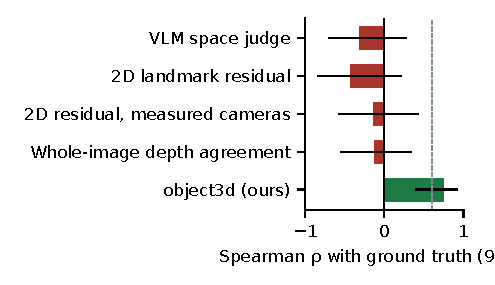
\includegraphics[width=\columnwidth]{figs/judges.pdf}
\caption{Scene-level agreement of each judge with ground truth on interiors. The dashed line marks the acceptance bar $\rho=0.6$.}\label{fig:judges}
\end{figure}

\section{A measured layout judge}\label{sec:object3d}
\paragraph{Measured cameras.} Monocular geometry fixes most of what the planner guessed. MoGe-2~\cite{moge2} intrinsics read the
reference vertical field of view to within about $2^\circ$ (per-view $\rho=0.95$ with the true error, also on centre crops of known zoom).
Depth Anything~3 relative pose brings the two views' relative rotation from $12.0^\circ$ (median; up to $79^\circ$) to $2.2^\circ$. MoGe-2 also
gives the first camera's height ratio (error 37\% $\to$ 5\%) and pitch ($2.9^\circ \to 0.4^\circ$). The pipeline locks these values when it
renders the reference views.
\paragraph{object3d.} For each observed landmark-view, $p_g$ is the median ray hit on the landmark's bound instances on a $64\times48$
grid, and $p_m$ is the median MoGe-2 point inside the inner half of the landmark's observation box. One scale per view,
$s=\mathrm{median}\,\|p_m\|/\|p_g\|$, makes the comparison scale-free, and the error is $\min(1,\|s\,p_g-p_m\|/\|p_m\|)$. An invisible
bound instance scores 1, and the scene score is the mean. The judge is deterministic, needs no model call, and runs in seconds.
\paragraph{Validation.} The observation boxes are mostly usable: 63\% of scored object-views are covered at IoU $\ge 0.5$, with a median best
IoU of 0.69. Against label-free truth (Fig.~\ref{fig:perlm}) object3d reaches $\rho=0.84$ $[0.74,0.90]$ over 203 landmark-views. With
unlocked cameras it is $0.84$, and the oracle that substitutes ground-truth depth for MoGe-2 reaches $0.86$, so the monocular point map
costs little. Per scene it reaches $0.75$ $[0.40,0.91]$ (18 scenes; $0.82$ over 34 recorded rounds from several pipeline variants). It ranks
11 of 12 interior perturbations correctly, and it catches the push that is invisible from view 1. On 13 graybox rounds generated
\emph{after} validation it still agrees with truth ($\rho=0.79$).

\begin{figure}[t]\centering
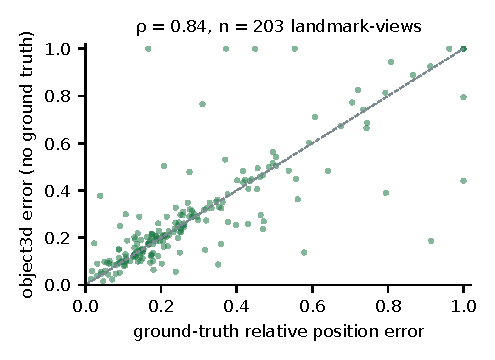
\includegraphics[width=\columnwidth]{figs/per_landmark.pdf}
\caption{object3d error, computed without ground truth, against label-free ground-truth error per landmark-view (camera-locked first rounds of 18 interiors).}\label{fig:perlm}
\end{figure}

\section{Closing the loop}\label{sec:loop}
We deployed object3d as the graybox acceptance gate under a per-job policy, so recorded jobs replay unchanged. A round passes when
object3d $\le 0.35$, every critical landmark is visible, the layout is not mirrored, and the reference cameras can move without hitting
geometry. The VLM review still runs, but only as repair feedback. Candidate selection and plateau detection follow object3d. The repair
feedback lists the worst landmarks with whether each sits too near or too far, and, for invisible ones, where they project now and where
the reference puts them.
\paragraph{Defects surfaced by a trustworthy gate.} Live runs exposed pipeline faults that the old judge had hidden:
\begin{itemize}\setlength\itemsep{1pt}
\item Reference frames were bound twice, and because the measured locks are not idempotent, every repair preview failed.
\item Repairs edited cameras that were locked by measurement, so the edits had no effect.
\item The clearance check toured the planner's cameras instead of the locked ones that render.
\item Recovery after a failed repair always failed.
\end{itemize}
\paragraph{Result.} On the hardest interior, which the pipeline had never accepted, the first fixed run passed in one repair round:
object3d fell from 0.81 to 0.33, and ground truth confirms the improvement (0.77 $\to$ 0.23; Fig.~\ref{fig:loop}). A second scene passed at
round 0 with anchored recall 0.73, its best result in any run.

\begin{figure}[t]\centering
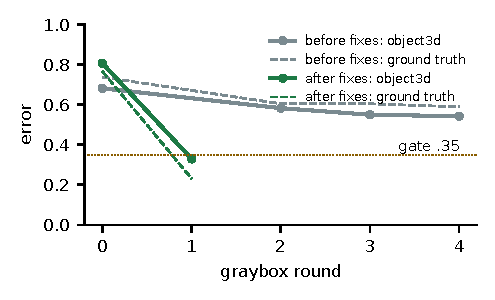
\includegraphics[width=\columnwidth]{figs/closed_loop.pdf}
\caption{Graybox repair on the hardest interior before and after the deployment fixes: object3d (solid) and label-free ground truth (dashed).}\label{fig:loop}
\end{figure}

\section{Orthographic scenes}
Every voxel reference is isometric. In an orthographic view an object's image size does not change with depth, and one view's depth
direction is a lateral direction in the other, so the 2D landmark checks already constrain 3D position. The existing objective gate ranks
all 80 known-worse variants correctly (depth shift along view 1, $15^\circ$ rotation, $1.3\times$ scale, 30\% dropped), and ground truth
agrees in 56 of 60 measured pairs. Its 0.10 residual limit is loose: it rejects only 1--3 of 20 of the milder variants. We keep it,
because correct layouts on real voxel references reach 0.086.

\section{Limitations}
The study covers 18 interiors, one generation pipeline and one VLM judge, and live deployment covers only a handful of scenes. Whether
VLM judges run against 3D truth across other models and generators is the main open question. The 0.35 gate threshold was set on the
same interiors. object3d depends on the pipeline's landmark observation boxes, which are poor in 2 of 18 scenes. It inherits the
behaviour of the monocular model, and it is untested on outdoor perspective scenes. End-to-end delivery quality under the new gate is
being measured. \todo{scale to 60--100 Hypersim scenes; add 2--3 open VLM judges; compare with MEt3R- and FurnSet-style scores; run
the gate on outputs of public generators; add a small human ranking study; report end-to-end delivery rates.}

\section{Conclusion}
A VLM that looks at reference and render can be confidently and consistently wrong about 3D layout, because image-plane agreement
does not imply 3D agreement. Judges for image-conditioned scene generation should be validated against per-object, label-free truth
before they gate or steer generation. A simple measured judge built from monocular geometry passes that test, and it makes an
agentic repair loop converge toward layouts that ground truth confirms. Code, benchmark and validation scripts will be released.

{\small\bibliographystyle{plainnat}\bibliography{refs}}
\end{document}
